\chapter{Results}
\label{chapter:results}

In this Chapter we present the results of our Langevin solver presented in the
previous chapter.
At first, we summarize the hardware and software tools we use for our experiments, then
we introduce the reference implementation of a Vlasov-Poisson solver that pursues a different
approach for modeling collisions.
We continue with a section where we test the collisionless solver, followed by a thorough
examination of both collisional terms (friction and diffusion) by means of the analytical test case from Section
\ref{section:test_cases}.
Lastly, we apply our Langevin solver to the \gls{dih} problem and investigate the
computed collisional terms.
Throughout this Chapter we refer to our implementation as ``Langevin solver'', regardless of its
experiment type (i.e. with or without collisions).

\section{Simulation Setup}
\label{section:simulation_setup}

The solver was programmed entirely in C++. For post-processing we use Python.
We use the Independent Parallel Particle Layer (\gls{ippl}) \cite{IPPL}, providing many tools and data structures instrumental to \gls{pic} codes such as ours.
Through the usage of the Kokkos Performance Portability Ecosystem \cite{trott2021kokkos}
we achieve hardware independent code. Meaning, we can compile our code for a multitude of computing
hardware (CPU, GPU, \dots) without requiring changes to the code itself.

The default experiment type uses a mesh size of $256^3$ and $64^3$ for discretizing the
configuration and velocity space, respectively (denoted by $[256]^3$, $[64]^3$ in the figure labels).
We choose to use periodic boundary conditions in configuration space to facilitate a direct
comparison between our \gls{pic} solver and Ulmer's.
As Ulmer correctly states, this is a reasonable assumption due to the large ratio between the chosen
box length and the sphere radius (see \ref{appendix:ulmerParams}).
In velocity space we use open boundary conditions, as motivated in Section \ref{section:rb_discretization}.
Due to the velocity domain being fairly large we found that Hockney's method was not able to
converge to an acceptable solution for the Rosenbluth potentials given our chosen mesh size.
This is why we applied domain normalization to $[-1,1]$ in order to solve for the Rosenbluth potentials.
If there are cases where we deviate from this setup we will state it explicitly.
Further simulation parameters are listed in Appendix \ref{appendix:ourParams}.

We run our experiments on a cluster of the Paul Scherrer Institut containing Nvidia GDX A100 GPUs.
Each unit has 40GB of memory and works in conjunction with an AMD Rome 7742 CPU
with 1 TB of system memory.
An experiment of the Langevin solver for 5 plasma periods takes approx. 1 minute on this hardware.


\subsection{Disorder Induced Heating in a Cold Sphere}
\label{subsection:dih_coldsphere}

We strive to replicate the same benchmark case as in \cite{mitchell2015parallel} and
\cite{p3m_ulmer}.
This benchmark simulates a cold electron sphere with radius $R = 17.74\ \mu \text{m}$ containing $N_p = 156055$
electrons and produces a bunch density of $n_0 = 6.67 \times 10^{18}\ \text{m}^{-3}$.
The bunch is initially at rest (zero velocity distribution), but quickly starts to expand due to the
self-generated electric field.
By applying a linear focusing force given by the average electric field multiplied by a focusing factor
$f_c = 1.5$, we can restrict this expansion and cause it to approach an equilibrium state.
Given the aforementioned properties of the system, the plasma oscillates at a frequency
of $\omega_p = 1.45 \times 10^{-11}\ \text{s}^{-1}$, equating to a period of 
$\tau_p = 4.31 \times 10^{-11}\ \text{s}$.
Mitchell \cite{mitchell2015parallel} states the analytical value for the normalized emittance
in this equilibrium as being $\neps^{\text{eq}} = 0.491\ \text{nm}$.
We choose to run our experiments for 1000 timesteps over 5 plasma periods.
This results in a timestep size of $dt = 2.15623\times10^{-13}\ \text{s}$, which coincides with the
one chosen by Ulmer \cite{p3m_ulmer}.

In Figure \ref{fig:emittance_p3m} we show the normalized emittance for varying $r_c$ for the
\gls{dih}
problem using the \gls{p3m} method. It is evident that considering a larger neighborhood for the
\gls{pp} interaction pushes the
fluctuating normalized emittance to the expected value of $\neps^{\text{eq}} = 0.491\ \text{nm}$.

In the subsequent sections of this chapter we refer to this benchmark solely as the ``\gls{dih} problem".


\begin{figure}
    \begin{center}
        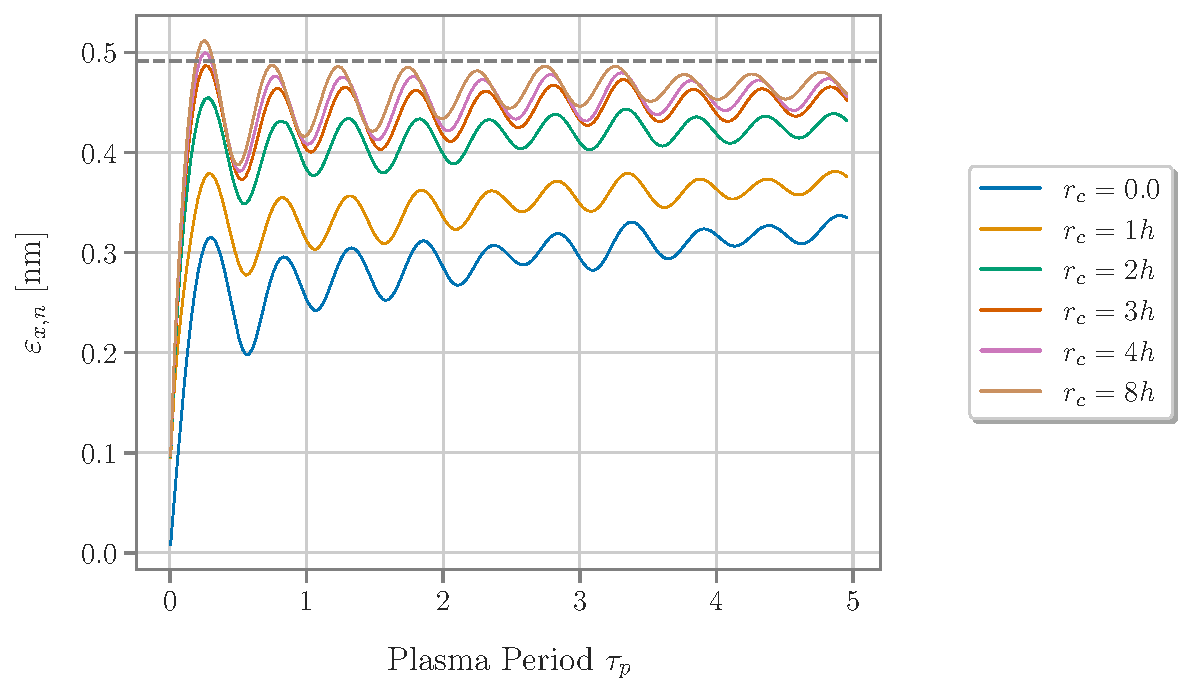
\includegraphics[width=0.80\textwidth]{figures/results/emittance_p3m.pdf}
    \end{center}
    \caption{Normalized emittance computed by the \gls{p3m} method \cite{p3m_ulmer} for varying cut-off radii $r_c(h)$,
    where $h = 0.39 \mu\ \text{m}$ is the mesh width. The dashed gray line signifies the expected limit for the normalized emittance.}
    \label{fig:emittance_p3m}
\end{figure}



\section{Collisionless Simulation}

In the following section we analyze a few selected statistics of our collisionless solver to ensure
that the implementation of the \gls{dih} problem functions as expected.

At first, we show that the average Lorentz factor for the \gls{dih} problem stays close to 1 (see Figure
\ref{fig:gamma_test}), meaning that the particles remain in the non-relativistic regime over the
course of the considered time frame of 5 plasma periods.
This indicates that we choose an appropriate focusing strength ($f_c = 1.5$) that keeps the
particles inside the computational domain.

\begin{figure}
    \begin{center}
        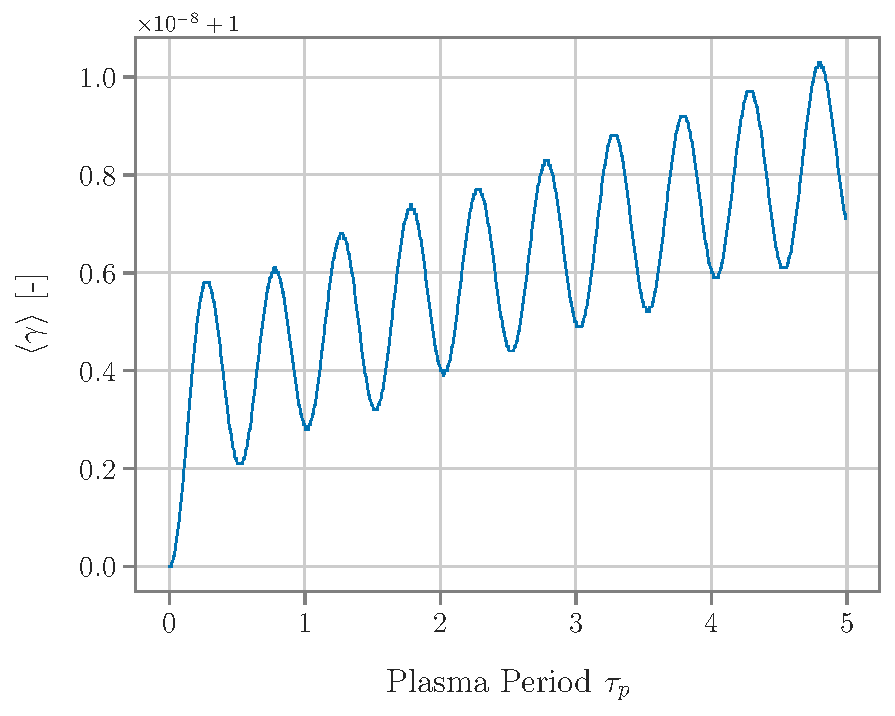
\includegraphics[width=0.60\textwidth]{figures/results/gamma_test.pdf}
    \end{center}
    \caption{Ensemble averaged Lorentz factor $\gamma$. Note the multiplicative factor of $\times
    10^{-8}$ shown at the top left corner. Plasma period $\tau_p = 4.31 \times 10^{-11}\ \text{s}$.}
    \label{fig:gamma_test}
\end{figure}

As we have seen in Table \ref{table:langevinPossibleMethods}, the Langevin solver can consist of
any combination of the given sub-methods.
We shall now analyze a subset of combinations in the electrostatic \gls{pic} solver.
The emittance values shown in Figure \ref{fig:EfieldGradientTest} appear to be impacted heavily by
how we choose to solve for the potential $\phi(\vect r)$, as well as the way we compute its gradient.
It comes unexpectedly that the Langevin-II solver in conjunction with a spectral gradient
computation ($\spVelNabla$) shows an upwards trend, and even surpasses the expected
limit of normalized emittance $\neps^{\text{eq}} = 0.491\ \text{nm}$.
Apart from this behavior, it agrees very well with the analytical value of the plasma period $\tau_p$.
The Langevin-II type solver generally results in larger amplitudes whereas the Langevin-I appears to
be more damped.
Nevertheless, it is hard to judge which combination results in the most ``correct" behavior 
of the emittance. Also, Ulmer's results have to be considered as just
an approximation of the correct behavior.

Thus, we would like to conclude that the choice of these two building blocks has a non-negligible
impact resulting in strongly different behaviors for a longer simulation time.
We suggest further investigation along these lines if one is interested in a solver optimally
tuned for the \gls{dih}
problem.
The justification for this decision is, that we would be able to observe an impact of Coulomb 
collisions on the normalized emittance irrespective of the chosen structure of the electrostatic
\gls{pic} solver.

The choice of the appropriate mesh size can also prove to be delicate, as we have to find a trade-off between a small
enough mesh width $h$ to resolve small-scale effects and given memory or compute time constraints.
It can be seen in Figure \ref{fig:meshsize_test_VICO} that a spatial discretization of size $256^3$ is
necessary for both solvers to show the oscillatory behavior we expect in the normalized emittance.

\begin{figure}[h]
      % \hspace*{-1cm}
  \begin{subfigure}[b]{0.535\textwidth}
    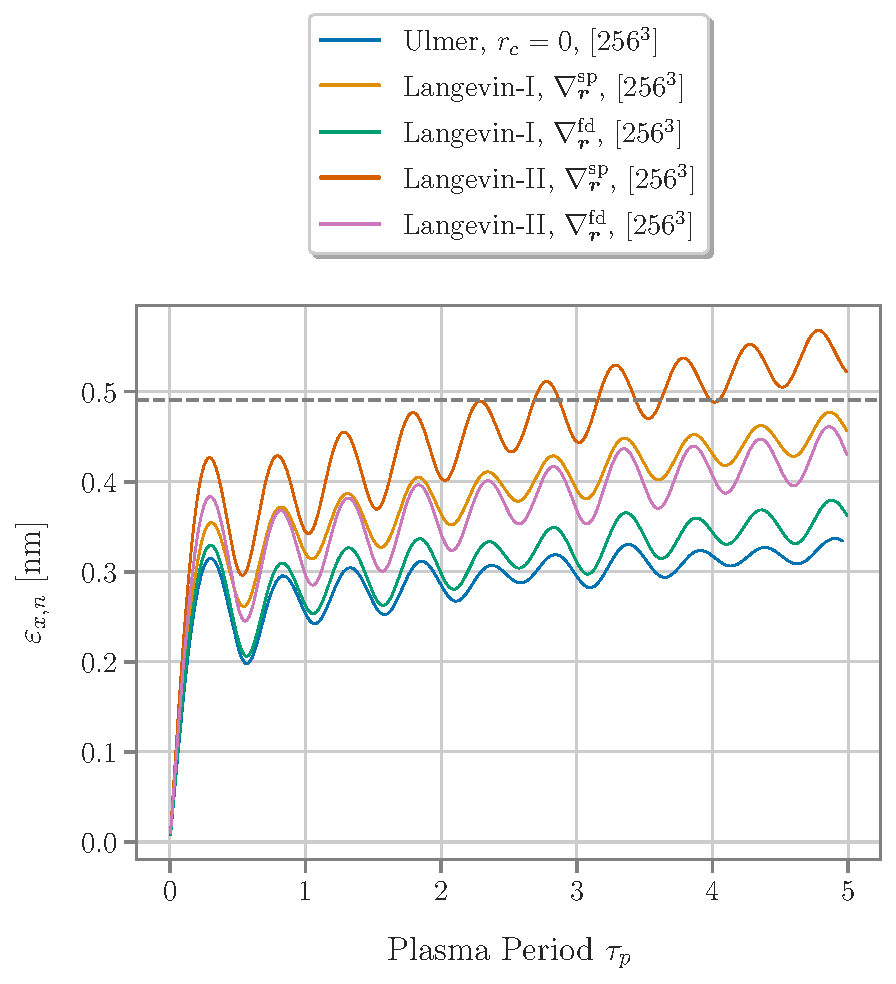
\includegraphics[width=\textwidth]{figures/results/Efield_gradient_test.pdf}
    \caption{}
    \label{fig:EfieldGradientTest}
  \end{subfigure}
  \hfill
  \begin{subfigure}[b]{0.548\textwidth}
    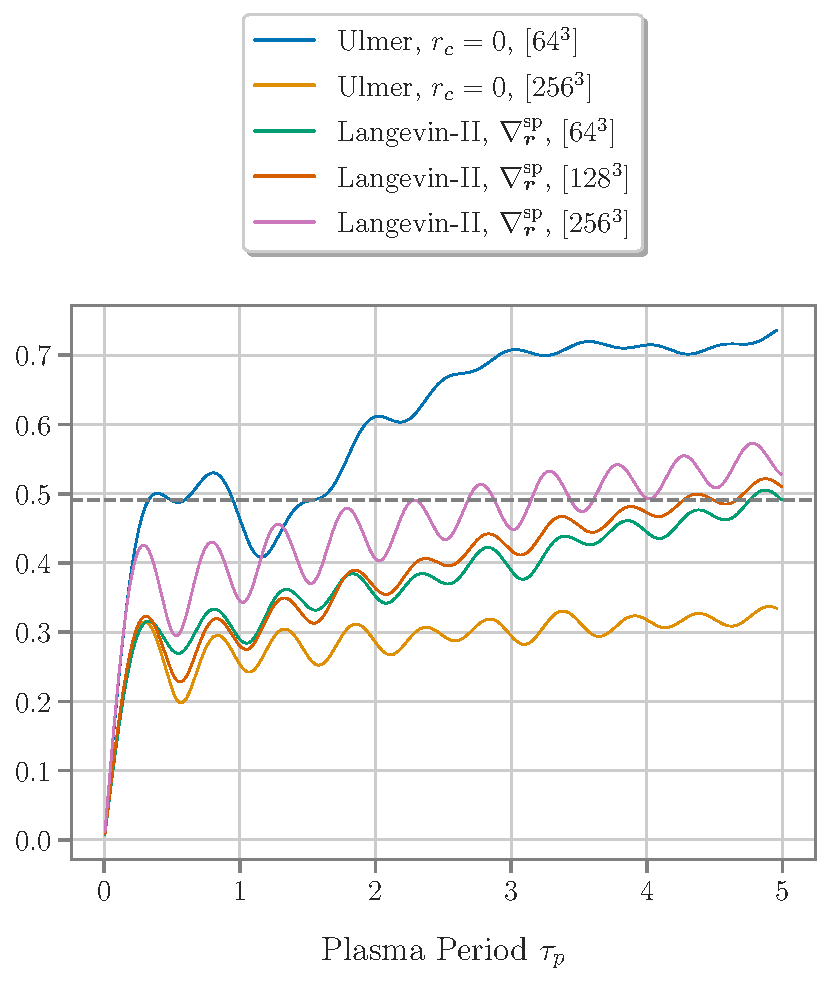
\includegraphics[width=0.9\textwidth]{figures/results/meshsize_test.pdf}
    \caption{}
    \label{fig:meshsize_test_VICO}
  \end{subfigure}
  \caption{Study on how the Poisson solver type impacts the normalized emittance $\neps$
      (\ref{fig:EfieldGradientTest}). Impact of varying spatial discretization on normalized
      emittance computed by the reference \gls{p3m}
      solver \cite{p3m_ulmer} ($r_c=0.0$\ cm) and the Langevin electrostatic \gls{pic} solver
(\ref{fig:meshsize_test_VICO}). The dashed horizontal line indicates $\neps^{\text{eq}}$.}
\label{fig:DIH_collisionless}
\end{figure}

\section{Gaussian Test Case}

With the formulations in Equations \ref{eq:gaussian_sols} we are able to test individual components
arising from the Rosenbluth potentials and to verify their correctness on 
an initial velocity density distribution given by Eq. \ref{eq:gaussian_pdf}.
We choose initial conditions that are similar to a snapshot of the three-dimensional velocity distribution 
at iteration 100 ($t = 0.0215\ \text{ns}$) of the \gls{dih} problem as then we expect the collisions to be a
dominant contribution to the system dynamics. The resulting velocities are sampled from $\mathcal
N(0, \sigma)$ with $\sigma = 0.05v_{max}$.

The potentials were solved for with Vico's method and exhibit a consistent order 2 convergence of the
relative error (see Figure \ref{fig:convergence_hg_VICO}). 
The same holds for Hockney's method (Appendix \ref{appendix:convergenceStudy}).
This might come as a surprise as we expect exponential convergence for Vico's method. But as
mentioned in Subsection \ref{subsection:vico} this only holds for sufficiently smooth functions.
In our case this is not given as on the one hand, our particle distribution is peaked around the
origin and on the other, we use the particle scatter operation to obtain the particle density in velocity space.
This causes a non-smooth density due to the finite mesh size and particle number.
Although we could either increase the particle density or use a higher order interpolation method
(for the scatter/gather operations) for further smoothness, the computation would quickly become too expensive 
in terms of memory usage and computation time.
This is mainly the case for the computation of the $\matr Q$ term as it requires multiple temporary data structures.

So far we cannot conclusively say which method is preferable. Regardless, we propose to
use Vico's method to be on the safe side. If one would ever encounter a smoother velocity
distribution (i.e. due to the aforementioned improvements to the \gls{pic} routines), the method
will show better convergence. Conveniently, it also exhibits similar computational complexity as Hockney's
method.

Hereafter we may only consider results computed with Vico's method to avoid distracting the reader with too many figures for both solver types.
We will state explicitly if there is some data that nonetheless used Hockney's 
method due to the results bearing unexpected or interesting behavior.

Having shown the expected convergence rate of the potentials we can move on and check it for the
individual collisional coefficients, $\vect F_d$ and $\matr D$.

\begin{figure}[h]
  \begin{subfigure}[b]{0.52\textwidth}
    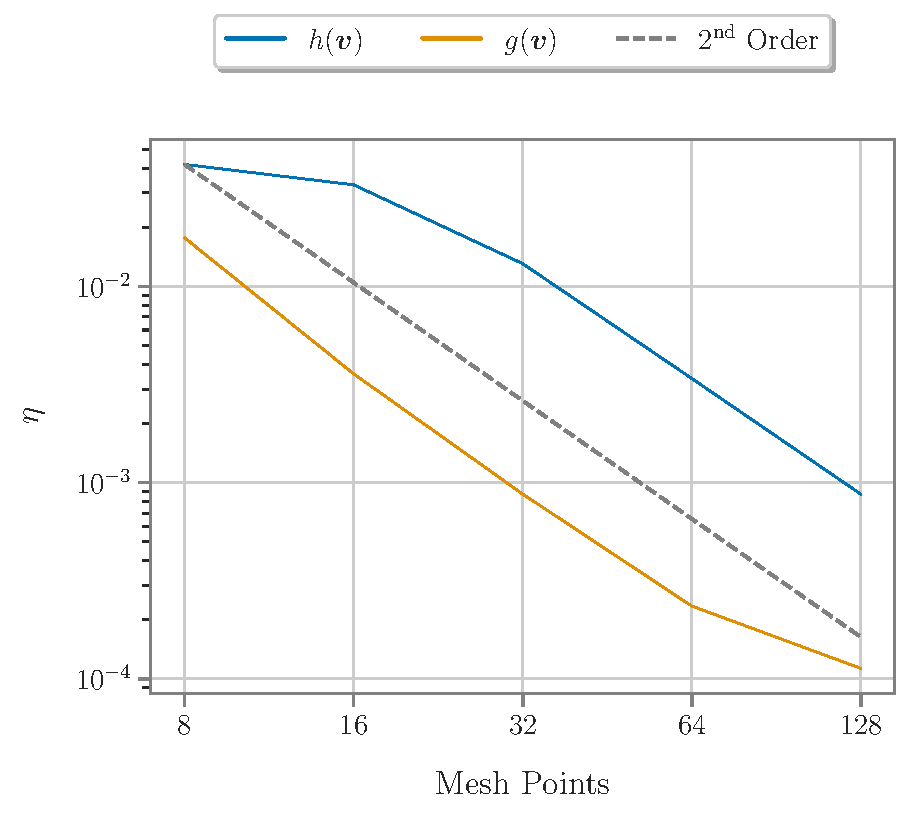
\includegraphics[width=\textwidth]{figures/results/convergenceStudy/hg_005vmax_VICO.pdf}
    \caption{}
    \label{fig:convergence_hg_VICO}
  \end{subfigure}
  \hfill
  \begin{subfigure}[b]{0.52\textwidth}
    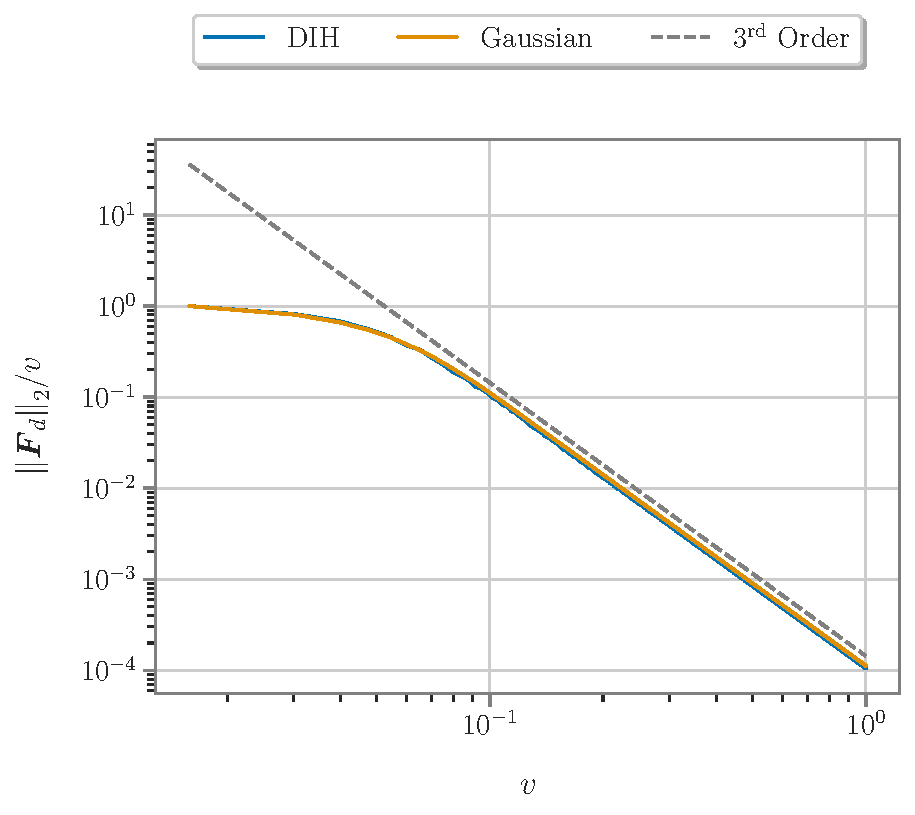
\includegraphics[width=\textwidth]{figures/results/Fd_asymptotic.pdf}
    \caption{}
    \label{fig:asymptoticFd}
  \end{subfigure}
  \caption{Convergence study of Rosenbluth potentials  solved with Vico's method (\ref{fig:convergence_hg_VICO}).
      The normalized friction coefficient distributions for both the Gaussian test case and the
      \gls{dih} problem after 
  5 plasma periods (\ref{fig:asymptoticFd}) exhibit the expected asymptotic $1/v^3$ fall-off (dashed gray line).}
\label{fig:convergence_VICO}
\end{figure}

\subsection{Friction \& Diffusion Coefficient}

At first, we are interested in how the values of the friction coefficients are distributed. We expect large
friction terms for small deflections/scatterings. Furthermore it should decrease at
an asymptotic rate of $1/v^3$ at large scatterer velocity as specified by \cite{manheimer1997langevin}.
The expected asymptotic fall-off is distinctly visible on a normalized log-log scale in Figure \ref{fig:asymptoticFd}.
The same behavior has been observed by Qiang et al. \cite{qiang2000self} (cf. Figure 4) for their specific test case of a
Maxwellian velocity distribution.

As for the convergence (Figure \ref{fig:convergence_VICO_spectral_FD_comparison}): $\vect F_d(\vect v)$ shows a similar order 2 error
convergence,
but we observe a difference for computing $\matr D(\vect v)$ with finite difference or with the
spectrally accurate method via the Fourier transform (as a byproduct of the computation of the Rosenbluth potential itself).
Interestingly enough the spectral computation performs worse, at least for this case of the velocity
distribution.
After increasing our mesh size above $64^3$ grid points, especially the accuracy of the diagonal elements of the Hessian
starts to deteriorate.
We point to the fact that the issue might lie in the actual magnitude of the values.
Altough, without further investigation of this behavior, choosing the finite difference approximation of the
Hessian is encouraged.
It is important that the the diagonal elements are computed correctly since they 
have been shown to be dominant in magnitude \cite{manheimer1997langevin}.
Due to runtime considerations we opt to use $64^3$ as our default mesh size in velocity space.
We follow up on the unexpected behavior of the diffusion coefficient with a more in depth analysis in Section \ref{subsection:diffCoeff}.

\begin{figure}[h]
  \begin{subfigure}[b]{0.52\textwidth}
    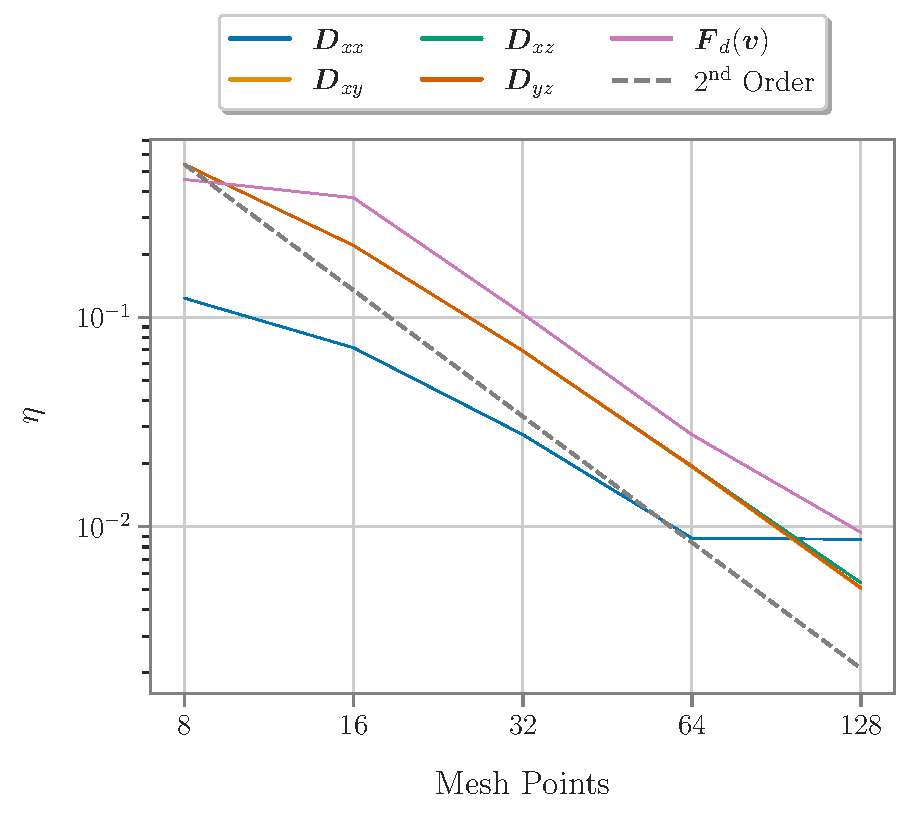
\includegraphics[width=\textwidth]{figures/results/convergenceStudy/D+Fd_005vmax_VICO.pdf}
    \caption{Finite Difference computation of coefficients.}
    \label{fig:convergence_DFd_VICO_FD}
  \end{subfigure}
  \hfill
  \begin{subfigure}[b]{0.485\textwidth}
    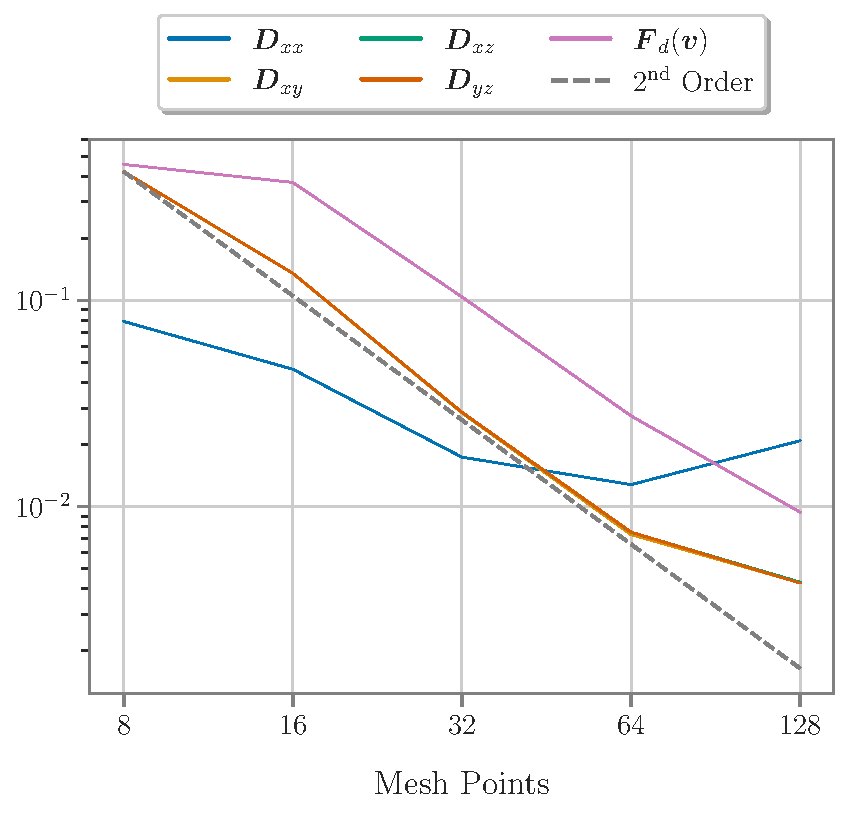
\includegraphics[width=\textwidth]{figures/results/convergenceStudy/D+Fd_005vmax_VICO_spectralHess.pdf}
    \caption{Spectral computation of coefficients.}
    \label{fig:convergence_DFd_VICO_spectral}
  \end{subfigure}
  \caption{Convergence study of collisional coefficients for a Gaussian
  velocity distribution which models the distribution of the \gls{dih} problem.}
\label{fig:convergence_VICO_spectral_FD_comparison}
\end{figure}


\subsubsection{Cholesky Decomposition}

We implemented the LDLT algorithm listed in Appendix \ref{appendix:LDLT} to achieve the Cholesky
decomposition of the Diffusion matrices $\matr D(\vect v)$.
Using the fact that for any real matrix $\matr A$, $\matr A \cdot \matr A^T$ is semi-positive definite, we
generated $10^4$ random semi-positive definite matrices and computed their decompositions.
We then compared it to the decompositions obtained with the SciPy \cite{2020SciPy-NMeth} Python 
module \texttt{scipy.linalg.ldl}. We found that all decompositions coincided.

\subsubsection{Coefficient Identities}

In Section \ref{section:rb_potentials} we derived identities that relate $\vect F_d$ and $\matr D$ with each other.
We observe the expected error convergence of second order for both identities (Figure
\ref{fig:identities_convergence_VICO}). Although it has to be
pointed out that the magnitude of the relative error values are large compared to the errors we
have encountered so far.
We also replicated this behavior by implementing it in Matlab \cite{MATLAB}. The code of this implementation
by A. Cerfon may be found on \cite{tobiaStudentRepo}.
We ascribe this to the repeated application of the numerical differential operators causing a non-negligible
accumulation of numerical errors.

\begin{figure}[h]
  \begin{subfigure}[b]{0.5\textwidth}
    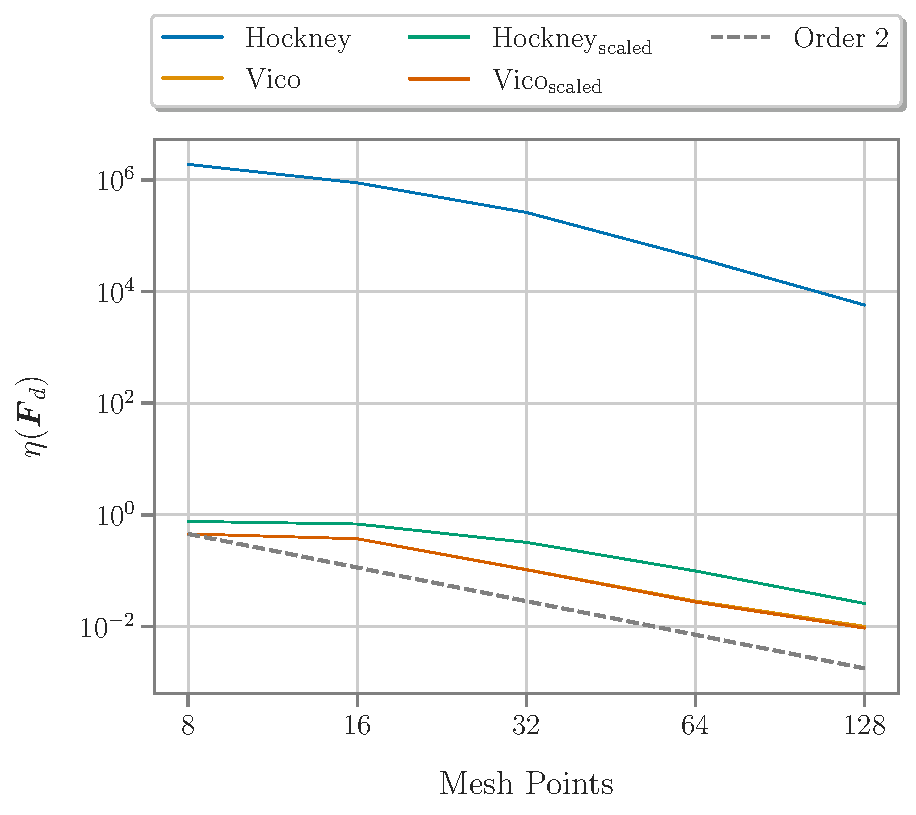
\includegraphics[width=\textwidth]{figures/results/convergenceStudy/Fd_joint_comparison.pdf}
    \caption{}
    \label{fig:Fd_joint_comparison}
  \end{subfigure}
  \hfill
  \begin{subfigure}[b]{0.524\textwidth}
    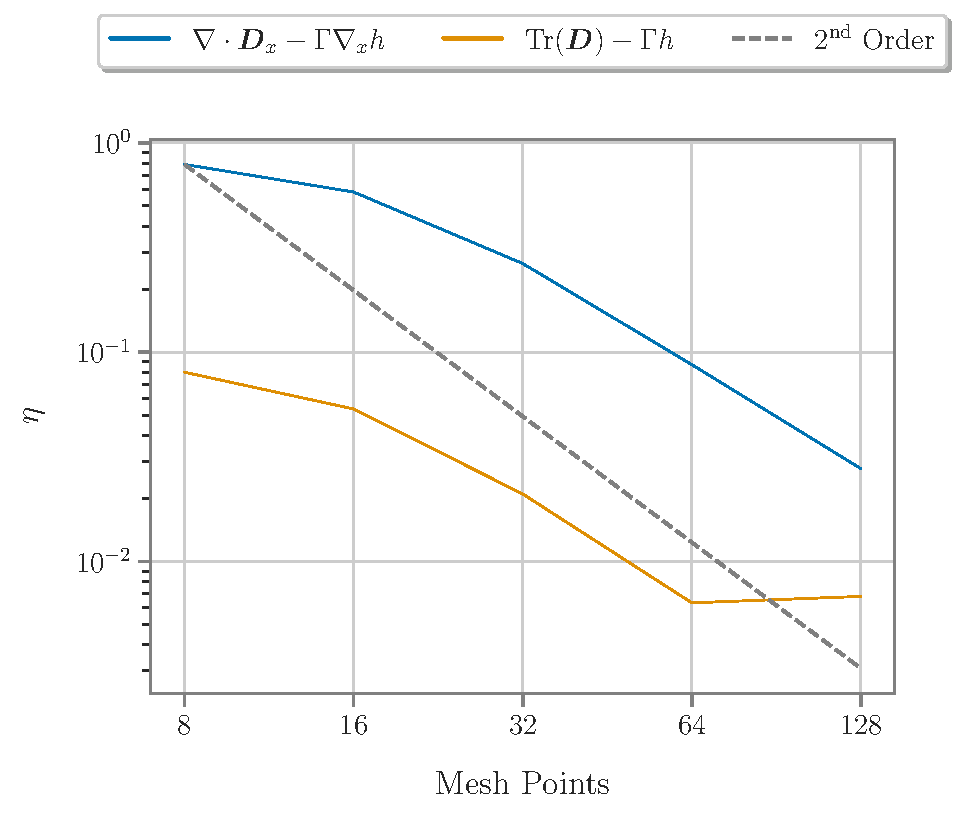
\includegraphics[width=\textwidth]{figures/results/convergenceStudy/identities_convergence_sigma005vmax_VICO.pdf}
    \caption{}
    \label{fig:identities_convergence_VICO}
  \end{subfigure}
  \caption{Unlike Vico's method, Hockney's method does not converge on the unnormalized
      (see subscript ``scaled")
  velocity space (\ref{fig:Fd_joint_comparison}). Convergence study of the identities defined
in Eq. \ref{eq:rb_identities} computed with Vico's method (\ref{fig:identities_convergence_VICO}).}
\label{fig:joint_Fdconvergence_identities}
\end{figure}

\section{Simulation with the Collision Operator}
\label{section:sim_with_collisions}

Following the thorough study of potential combinations of solver components outlined in the
preceding sections, we opt to employ the solver setup as stated in Table 
\ref{table:DIHsolverCombination} for the subsequent experiments on the \gls{dih} problem.

\begin{table}
    \renewcommand*\arraystretch{1.5}
    \centering
    \caption{Solver setup for the \gls{dih} experiments.}
    \label{table:DIHsolverCombination}
    \begin{tabular}{|l|l|l|}
\hline
\textbf{\gls{pic} Type}                           & \textbf{Quantity of Interest}
                                            & \textbf{Comp. Domain or Method}     \\ \hline
\multirow{2}{*}{Electrostatic \gls{pic}} & $\phi(\vect r)$
                                   & Definition I                 \\ \cline{2-3} 
                                   & $- \posNabla \left[ \phi(\vect r) \right]$
                                   & Spectral Gradient: $\spPosNabla$          \\ \hline
\multirow{2}{*}{Velocity \gls{pic}}      & $\velNabla h(\vect v)$, $g(\vect v)$                                        
                                   & Vico + $\spVelNabla$                       \\ \cline{2-3} 
                                   & $\frac{\partial^2}{\partial \vect v \partial \vect v} g(\vect v)$
                                   & \gls{fd} Hessian: $\fdVelHess$           \\
\hline
\end{tabular}
\end{table}

In the course of this investigation we encounter several unexpected outcomes which we each address and 
try to give the reader an intuition as to why this might be the case.

\subsection{Friction Coefficient}
\label{subsection:friction_coefficient}

The Gaussian test case provided us with two important insights: $\vect F_d$
indeed exhibits the correct distribution (Fig. \ref{fig:asymptoticFd}) and one needs to normalize
the velocity domain in order to observe the correct values (Fig. \ref{fig:Fd_joint_comparison}) with
Hockney's method.

The integration of the friction coefficient to the \gls{dih} time integrator as stated in Alg.
\ref{alg:integrator} does not appear to have an impact on the normalized emittance (Fig.
\ref{fig:Fd_DIH}).
The computed values are in the order of $10^{11}$ (Fig. \ref{fig:FdAvg_timeevolution}), which
is far too small to have an impact on the particle velocities during one timestep ($dt = 2.15 \times 10^{-13}\ \text{s}$).
This finding is unexpected, given that in the previous section, we have demonstrated that the
friction coefficient matches well with the analytical solution of the test case.
Due to the two coefficients being closely related computationally, we address potential reasons for
the unexpected behavior after also having presented the results for the diffusion coefficient.

\begin{figure}[h]
  \begin{subfigure}[b]{0.49\textwidth}
    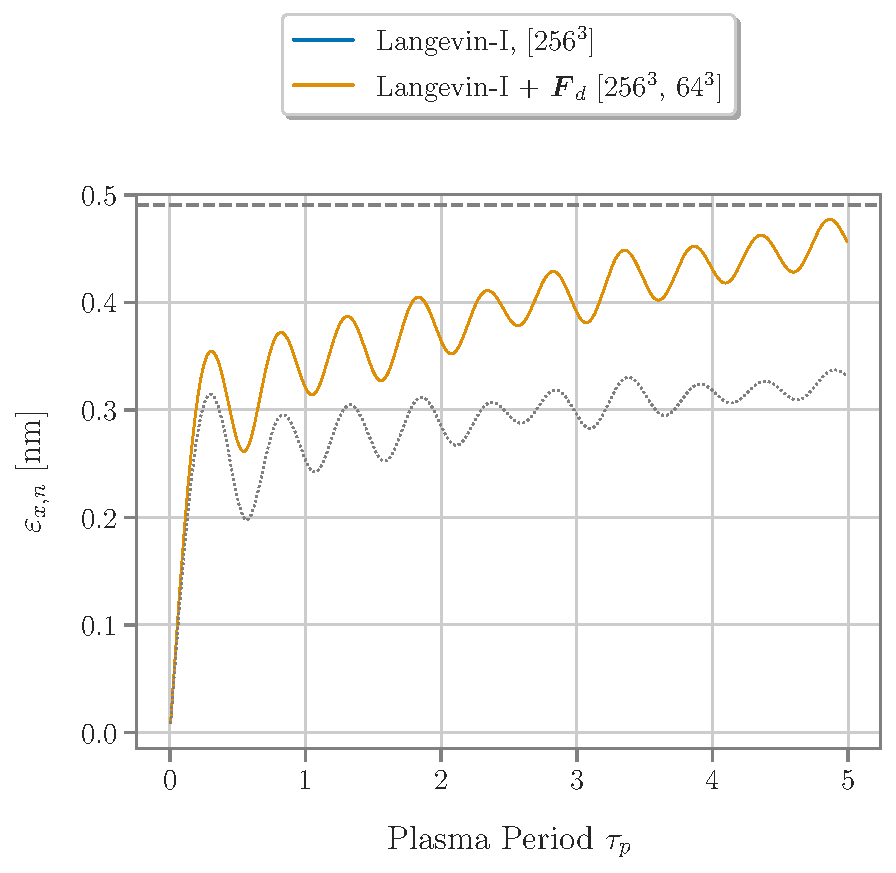
\includegraphics[width=1.0\textwidth, keepaspectratio, valign=b]{figures/results/Langevin_Fd.pdf}
    \caption{}
    \label{fig:Fd_DIH}
  \end{subfigure}
  \hfill
  \begin{subfigure}[b]{0.49\textwidth}
    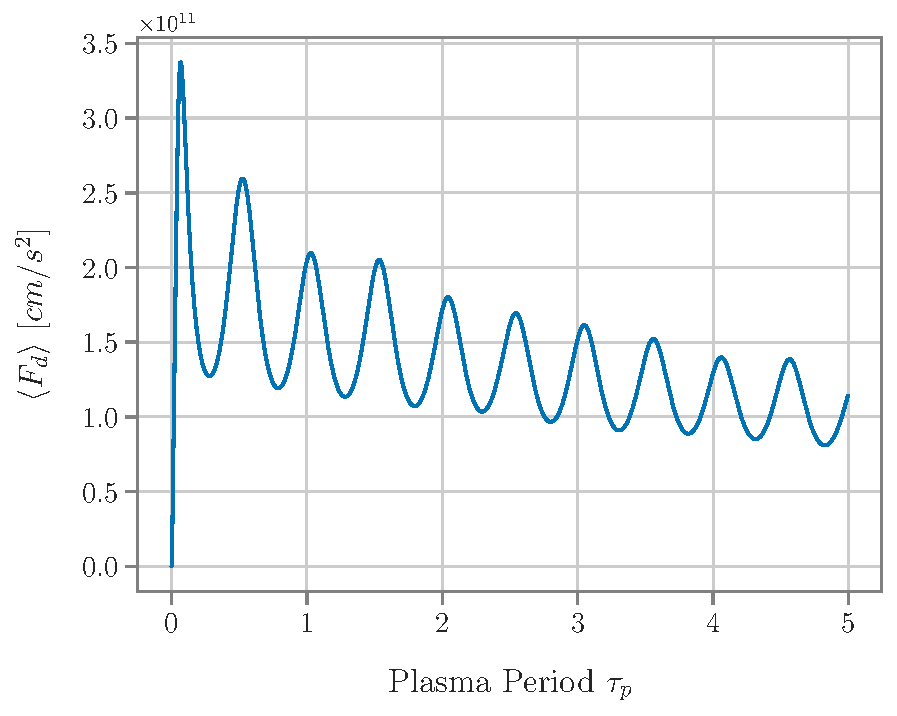
\includegraphics[width=1.0\textwidth, keepaspectratio, valign=b]{figures/results/Fd_avg.pdf}
    \caption{}
    \label{fig:FdAvg_timeevolution}
  \end{subfigure}
  \caption{Langevin simulation with friction enabled (\ref{fig:Fd_DIH}). The dotted line represents the
      emittance with Ulmer's collisionless solver and the dashed gray line the emittance limit. Average norm of the
  friction coefficient over 5 plasma periods (\ref{fig:FdAvg_timeevolution}).}
\label{fig:Fd_analysis_DIH}
\end{figure}

\subsection{Diffusion Coefficient}
\label{subsection:diffCoeff}

The computation of the diffusion matrix $\matr D$ works as expected. We plot the behavior
of the averaged first diagonal entry and the off-diagonal elements over 5 plasma periods (Fig. \ref{fig:Davg_timeevolution}).
Due to the coefficients being zero at $t = 0.0\ s$, we excluded the first 20 timesteps from the plot. 
This way we can better inspect the behavior after th initial warm up period.

This element-wise analysis confirms that the diagonal values  are indeed dominant as anticipated and show that they
attain a distinct periodic behavior already early in the simulation.
All diagonal elements of the diffusion matrix coincide due to the symmetry of the problem
(Fig. \ref{fig:Ddiag_avg}).
The off-diagonal elements show higher sensitivity to the initial conditions in form of noise. The
periodic behavior thus only starts to appear after 3 plasma periods.

\begin{figure}
  \begin{subfigure}[b]{0.49\textwidth}
    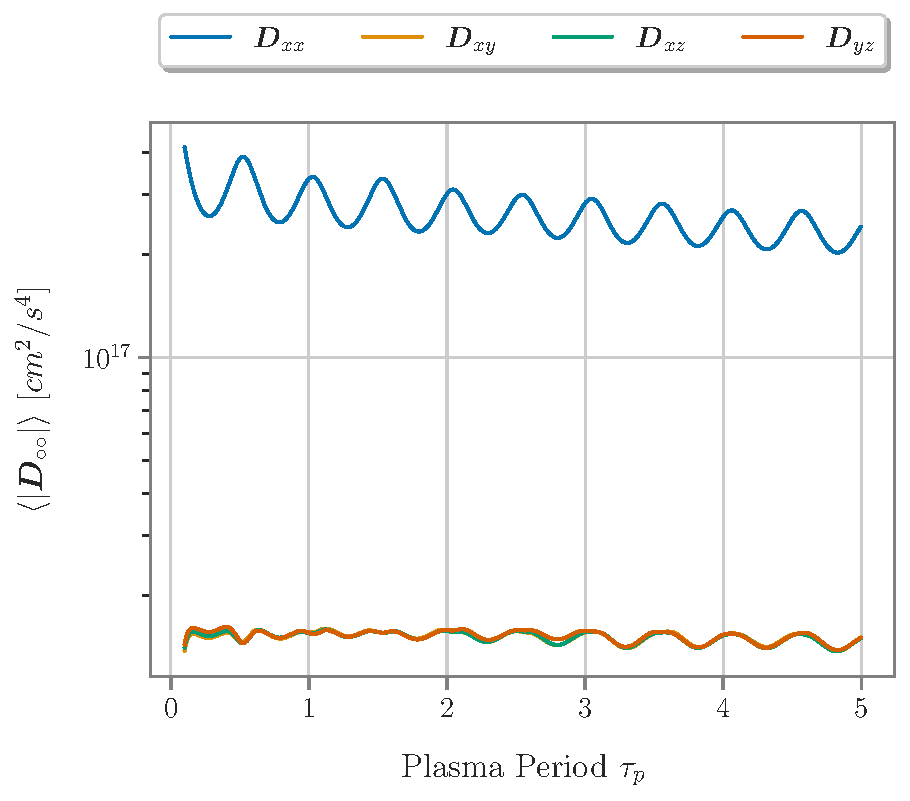
\includegraphics[width=\textwidth, keepaspectratio, valign=b]{figures/results/D_avg.pdf}
    \caption{}
    \label{fig:Davg_timeevolution}
  \end{subfigure}
  \hspace{2mm}
  \begin{subfigure}[b]{0.42\textwidth}
    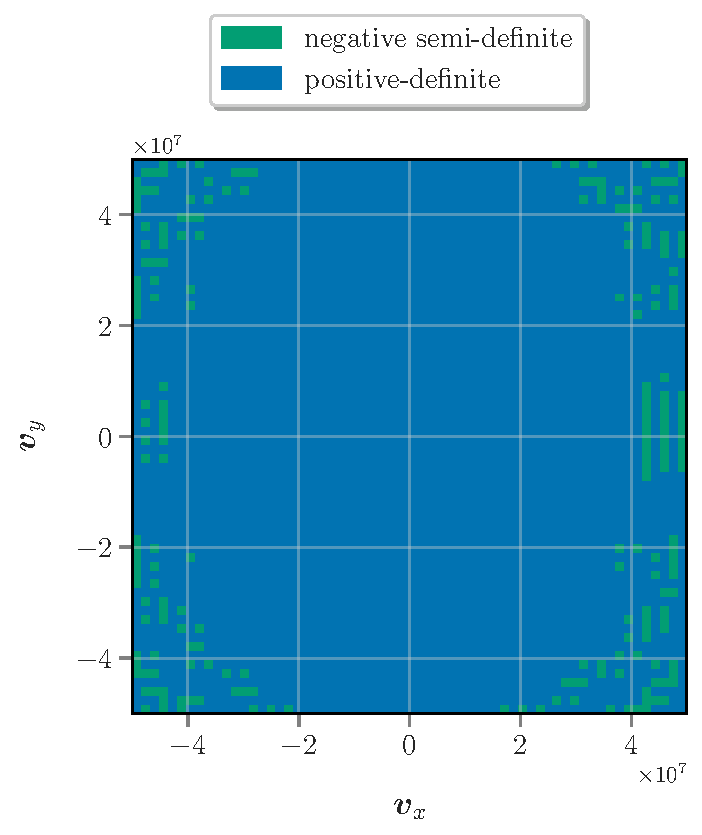
\includegraphics[width=\textwidth, keepaspectratio, valign=b]{figures/results/D_cholesky_it0800.pdf}
    \caption{}
    \label{fig:D_cholesky}
  \end{subfigure}
  \caption{Elements of computed diffusion coefficients over 5 plasma periods
  (\ref{fig:Davg_timeevolution}). Slice through the diffusion matrix field at $\vect v_z = 0$ 
and $t = 4 \tau_p$ indicating the matrix property for each entry (\ref{fig:D_cholesky}).}
\label{fig:D_analysis_DIH}
\end{figure}

Despite the promising results so far, we encounter issues when attempting to find a Cholesky
decomposition for the diffusion matrices at the particle locations.
Upon analyzing the matrices themselves, it turns out that a small number do not obey the semi-positive
definiteness property postulated in Section \ref{section:rb_potentials}.


We state the hypothesis that the property does not hold due to problems in our method and not the
mathematical proof being flawed.
Hence, we are interested to inspect in what cases the matrices are not semi-positive definite.

We take a snapshot of the matrix field at the last iteration ($t=5\tau_p$) and assign each entry a label according to
its matrix property.
In Figure \ref{fig:D_cholesky} we show a slice through this field at $\vect v_z = 0$ after 4 plasma
periods.
An unanticipated accumulation of negative semi-definite matrices emerges along the boundaries of the domain.
We might speculate that this has to do with the fact that we are using \gls{fd} to compute
$\matr D$.
This rationale is quickly refuted by comparison with a field computed with the spectrally
accurate Hessian which satisfies the open boundary conditions of the velocity domain 
(see \ref{fig:D_cholesky_spectralHess}).
In fact, these numerical remnants are even more pronounced for diffusion matrices computed with the 
Hessian of spectral accuracy.

When plotting these slices at periodic intervals of length $\tau_p$ (see Fig. \ref{fig:D_cholesky_time}), we observe that the halo of
negative semi-definite matrices starts to disappear after $t = 3\tau_p$.
This corresponds well with our previous observation of the off-diagonal elements reaching stable periodic behavior
after the first three plasma periods (Fig. \ref{fig:Davg_timeevolution}).
An additional finding, confirming the off-diagonals as the cause for some matrices not being
factorizable, is that the diagonal values of $\matr D$ are all positive.

\begin{figure}[!ht]
    \begin{center}
    \hspace*{-1.3cm}
        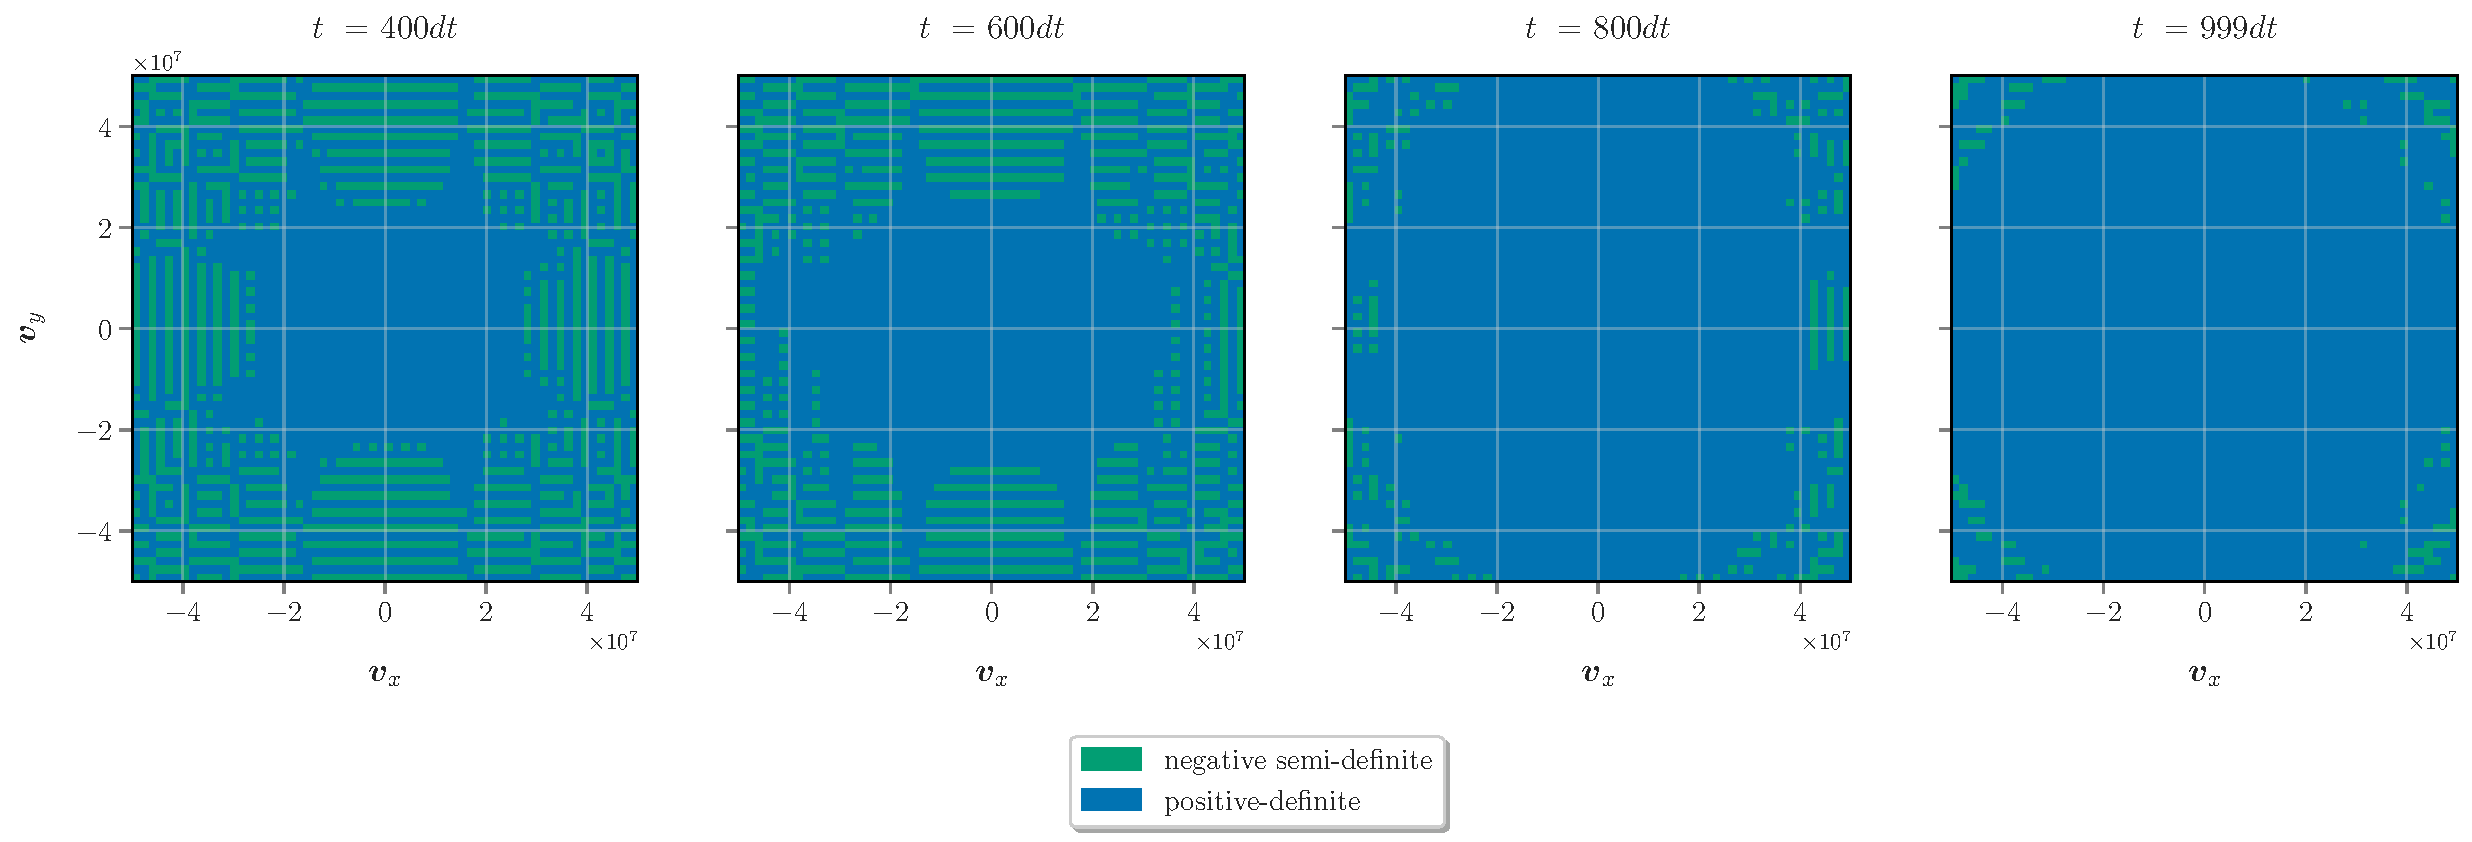
\includegraphics[width=1.18\textwidth]{figures/results/D_cholesky_time.pdf}
    \end{center}
    \caption{Evolution of a slice through the diffusion matrix field at $\vect v_z = 0$ over time.}
    \label{fig:D_cholesky_time}
\end{figure}

There exist a few plausible explanations for observing such behavior in the diffusion matrices.
The \gls{dih} problem starts from an initial condition (zero velocity distribution) which cannot be
assumed to be physical due to the discontinuity of Dirac delta function.
Therefore we expect the dynamics to behave in a way which may violate smoothness assumptions made on the diffusion tensor computation. 
After the system has started to come closer to the equilibrium state we see that this issue
disappears and our assertions hold.

The pattern which remains after 5 plasma periods appears to consist of concentric circles.
Since the probability distribution is peaked around the origin of the domain, and we consider a
one-to-one correspondence between macro-particles and electrons, the particle density can become
very small towards the boundaries.
Due to the large magnitude difference with respect to the density at the origin, it could then be that
solving for the Rosenbluth potentials introduces large relative numerical errors in the vicinity of the boundary.

\subsection{Summary}

We showed the correctness of our Langevin type collision operator for the \gls{fp} equation on
analytical test cases, demonstrating second order convergence for both the dynamical friction
$\vect F_d$ and diffusion term $\matr D$.

Subsequently we applied the operator on the cold sphere \gls{dih} problem stated in
\ref{subsection:dih_coldsphere} and found that the collisional effects introduced by the friction
coefficients being too small to impact the normalized emittance of the electron sphere.
The diffusion coefficients were shown to occasionally inhibit the decomposition necessary for the
time integrator due to negative semi-definiteness.
We observed that they exhibit large noise levels on the off-diagonal entries
over the course of the first three plasma periods after which they show a regular oscillatory behavior.
This change is also reflected in the definiteness property of the computed diffusion matrices, which
causes the number of negative semi-definite matrices to decrease drastically from this point onward.
We propose three possible explanations for the observed behavior of the collision coefficients:
\begin{enumerate}
    \item The \gls{dih} problem's initial condition (Dirac delta function at the origin) results in a
        discontinuity which does not conform with the assumptions made during the derivation
        of the Rosenbluth potentials. This is closely related to the next proposition.
    \item The current combination of timestep / mesh width does not allow to properly resolve the
        collisions in velocity space.
        The discontinuities at $t=0$ will cause numerical instabilities in the timestepping
        if the speed of the collision based relaxation cannot be accurately resolved within a
        timestep / cell in velocity space.
    \item The chosen number of macro-particles ($N_p=156055$) is too small to capture small-scale
        effects introduced by the collisions. As an example: considering a uniform distribution of the
        macro-particles, the test setup results in every cell containing on average less than 1
        macro-particle. The observation made in Figure \ref{fig:D_cholesky_time} shows that
        numerical errors are likely being introduced where few particles are present.
\end{enumerate}
